\pdfoutput=1
\documentclass{llncs}
\usepackage[T1]{fontenc}
\usepackage{newtxtext}
\usepackage[varvw]{newtxmath}
\usepackage{graphicx}
\usepackage{booktabs}
\usepackage{placeins}
\usepackage{amsmath}
\usepackage[hidelinks]{hyperref}
\pdfmapfile{+newtx.map}
\pdfmapfile{+qtm.map}
\pdfmapfile{+txfonts.map}
\pdfmapfile{+cm.map}
\hypersetup{pdftitle={Auditable Solar-Access Decision Support through Exact Blocker Reuse and Containment-Constrained Translation},pdfauthor={},pdfsubject={Anonymous regular-paper manuscript for author review},pdfkeywords={solar access, decision support, exhaustive screening, geometry validation},pdfcreator={LaTeX}}
\pdfinfoomitdate=1
\pdftrailerid{}
\newcommand{\aidraft}{~\cite{openai2026}}
\newcommand{\ind}{\mathbf{1}}
\begin{document}
\title{Auditable Solar-Access Decision Support through Exact Blocker Reuse and Containment-Constrained Translation}
\author{}
\institute{}
\maketitle
\begin{abstract}
Early-stage solar-access decisions require efficient comparison of interventions and reliable translation of simplified rules into geometry. We study a bounded decision-support workflow that selects two of 36 eligible building groups in a 45-building canonical model, giving 630 uniform-height-reduction candidates. Building-level occlusion reuse evaluates every candidate with the same ray--footprint primitive as repeated intersection, while a separate containment audit checks translated stepback solids. Across three matched single-thread repeats, full-universe median runtimes are 11,608.183~s for repeated intersection and 24.037~s for reuse, including precomputation, with equivalent pointwise exposure, metrics, scores, ranks and Pareto results. This 482.927-fold ratio applies to these two implementations, not to arbitrary solar-analysis software. Frozen same-site comparison cohorts of 23 and 20 candidates show strong aggregate agreement with archived Honeybee/Radiance results; the 20-candidate low-sun-area mean absolute error is 0.45~m$^2$, arising from one candidate-level difference of 9~m$^2$. Six controlled historical replays identify outside-footprint walls as the cause of adverse sunlight changes. Four separately simulated contained corrections remove those adverse events on the fixed grid and rays. The canonical geometry remains a component-bounding-box approximation with overlapping footprints. The contribution is an auditable computational screening and translation workflow, conditional on that model, rather than as-built validation or an automatically approved design. Drafting and editing assistance is disclosed for this abstract and the paper~\cite{openai2026}.
\keywords{Decision support \and Solar access \and Exhaustive screening \and Occlusion reuse \and Geometry containment}
\end{abstract}

\section{Introduction}
Early-stage changes to urban form pose a decision-support problem: planners need to compare many interventions, but a favorable simulation score is useful only if the evaluated geometry implements the intended change.\aidraft{} Solar-access screening therefore requires both an efficient evaluation procedure and an explicit check on the feasibility of translating a rule into a solid model. Here solar access means sampled outdoor direct-sun duration, distinct from irradiation, indoor daylight and annual energy performance~\cite{compagnon2004urban,czachura2022metrics}.

Two stages of a common workflow expose different risks. During screening, candidates that change only a small part of a scene repeatedly evaluate unchanged obstructions. During design translation, a nominally subtractive stepback may inadvertently place material outside the original building footprint. Faster ranking addresses the first problem but cannot resolve the second: an invalid translation can invalidate the premise of a favorable candidate without changing the correctness of its original score.

We study a deliberately bounded case: all 630 pairs from 36 eligible building groups in a 45-building canonical model. A fixed height-reduction rule defines each candidate; four reported metrics, a declared preference score and an area--volume Pareto analysis support comparison. The decision universe is fixed rather than learned or expanded adaptively. Eligibility is a research constraint, not permission to alter a property, and the canonical geometry is an approximate model rather than an as-built survey.

The paper makes three application-specific contributions:
\begin{enumerate}
\item An exact blocker-count update for the declared fixed-footprint rule universe, with explicit conditions for equivalence to repeated geometric intersection. Exactness concerns reuse of a common primitive, not physical ground truth or equivalence to another ray tracer.
\item A matched end-to-end implementation comparison that includes precomputation and checks pointwise exposure, metrics, scores, ranks and Pareto membership before reporting runtime. Frozen same-site Honeybee/Radiance comparisons provide a separate, qualified assessment of aggregate agreement.
\item A containment-based check on design translation, supported by controlled replays that locate historical adverse ray events and evaluate separately generated contained corrections. Failed historical outcomes remain visible, and geometric containment is distinguished from volume matching and professional feasibility.
\end{enumerate}
Together these contributions connect computational screening to a verifiable translation step. The objective is not a new general optimization algorithm, but evidence about when a reusable evaluation and a subtraction-based geometric interpretation are trustworthy within a declared model. The results address efficiency, cross-route agreement and translation validity separately; none establishes unrestricted solver superiority or automatic design approval.

\section{Related Work and Positioning}
Urban solar assessment relates built form to several distinct performance objectives.\aidraft{} Compagnon~\cite{compagnon2004urban} examines solar and daylight availability in urban fabric, while Czachura et al.~\cite{czachura2022metrics} organize solar-performance metrics for planning. These studies motivate an explicit choice of decision metric: the thresholded direct-sun-duration measure used here is not interchangeable with irradiation, daylight autonomy or a statutory compliance test.

Simulation-based building optimization provides a broader setting for repeated performance evaluation. Nguyen et al.~\cite{nguyen2014review} review its methods, applications and computational challenges. Konis et al.~\cite{konis2016passive} connect building form and passive-performance objectives, and De Luca et al.~\cite{deluca2021reverse} develop reverse solar-envelope form finding with regulatory constraints. Our search is narrower: a finite set of prescribed two-building reductions is exhaustively evaluated, then translated geometries are checked separately. We do not compare search efficiency or design quality against these broader form-finding approaches.

Computational reuse should also be distinguished from multifidelity modeling. Peherstorfer et al.~\cite{peherstorfer2018survey} survey methods that combine models of different cost and fidelity. In the present timing comparison, A and B use the same geometric primitive and solar vectors; B reorganizes identical blocker contributions rather than replacing the primitive with a lower-fidelity surrogate. The archived Honeybee comparison is a separate cross-route check, not a calibrated multifidelity estimator, and its effective solar vectors differ from those used by the screening route.

Performance ranking alone does not specify a satisfactory design decision. Mueller and Ochsendorf~\cite{mueller2015preferences} combine designer preferences with structural performance in conceptual design. Here the fixed score makes one declared preference ordering reproducible, while the area--volume Pareto view exposes a limited trade-off. Neither resolves ownership, construction, structural or regulatory constraints. Our containment test addresses a more basic prerequisite: whether the translated solid satisfies the subtraction premise under which sunlight cannot worsen on fixed rays.

Ladybug~\cite{roudsari2013ladybug}, Radiance~\cite{ward1994radiance} and pvlib~\cite{holmgren2018pvlib} supply environmental-analysis, ray-tracing and solar-modeling context. Their established roles do not validate this study's particular geometry or protocol. The contribution lies in keeping reuse equivalence, aggregate agreement, preference ranking and geometric feasibility distinct while connecting them in one auditable decision-support case.

\section{Decision Model and Exposure Estimator}
\subsection{Bounded Candidate Universe}
Let $\mathcal{B}$ denote the 45 building groups, each represented by a footprint $F_i$ and height $h_i$.\aidraft{} The eligible subset $E\subset\mathcal{B}$ contains 36 groups selected using source flags for movable and protected buildings, strict Boolean parsing and $h_i>3$~m. A feasible rule decision satisfies
\begin{equation}
 z_i\in\{0,1\}\ (i\in E),\qquad \sum_{i\in E}z_i=2,
 \label{eq:select}
\end{equation}
with $z_i=0$ outside $E$. For a selected building, the rule height is
\begin{equation}
 h_i^r=\max\{3,\ h_i-\min(3,0.25h_i)\},\qquad
 h_i(z)=(1-z_i)h_i+z_i h_i^r, \label{eq:height}
\end{equation}
where heights are in metres. Thus $\binom{36}{2}=630$ unordered pairs constitute the complete declared universe. Exhaustive evaluation establishes an optimum only for a specified score within this finite universe. It says nothing about other numbers of altered buildings, alternative height rules, footprint changes, structural feasibility or legal rights.

The canonical footprints are unions of bounding boxes associated with DXF components. Some building identifiers share components and some footprints overlap. The archived OBJ representation also disagrees with the canonical model for important candidates. We retain the frozen canonical input for reproducibility, but do not describe it as a surveyed or as-built boundary model. This distinction affects both visibility and volume interpretation.

\subsection{Receiving Grid, Time Samples and Visibility}
The protocol fixes 2,031 receiving points on a 3~m horizontal grid at height 0.1~m. The geographic parameters are latitude $24.55^\circ$N and longitude $118.03^\circ$E, with UTC+8 local time and an assumed north angle of zero. The declared analysis date for the pvlib sequence is 21 December 2026. Sixteen half-hour samples are centred at 08:15, 08:45, $\ldots$, 15:45. Each carries weight $\Delta t=0.5$~h, so the total integration weight is 8~h, despite the 7.5~h span between the first and last sample centres. These are discrete samples, not continuous-time exposure measurements.

For receiver $j$ and sample $t$, let $d_t=\ind\{\alpha_t>0\}$ indicate an above-horizon solar altitude and let $b_{jt}(z)$ indicate obstruction by at least one building. Direct-sun duration is
\begin{equation}
 D_j(z)=\sum_{t=1}^{T}\Delta t_t\,d_t\,[1-b_{jt}(z)].
 \label{eq:dsh}
\end{equation}
The geometric primitive intersects a horizontal ray with a footprint and uses the first positive projected distance $\ell$ to compare the ray height $0.1+\ell\tan\alpha_t$ against the building height. The source primitive ignores distances at most $10^{-7}$~m and uses a $10^{-9}$~m height tolerance. Point ordering, footprint construction, direction convention, tolerances and solar vectors are held identical in the matched comparison. The actual canonical case has no polygon holes; all receiving points were verified outside the canonical building footprints and off their boundaries. Those case-specific checks do not establish correctness for arbitrary polygon holes or boundary configurations.

The explicit active-sun factor in Eq.~\ref{eq:dsh} is important. A reproduced latent defect in the legacy routine skips constructing below-horizon rays but then counts their unblocked entries as visible. All 16 saved samples are above the horizon, so this defect is not evidence of a wrong frozen exposure value. It is nevertheless a reason to require an active-sun mask for extensions to other schedules.

\subsection{Metrics and Preferences}
Let $D_j^0$ be baseline duration, $P=2031$, $a=9$~m$^2$ the grid-area weight and $\tau=3$~h the research threshold. Four candidate metrics are
\begin{align}
 A(z)&=a\sum_j\big[\ind\{D_j^0<\tau\}-\ind\{D_j(z)<\tau\}\big],\label{eq:area}\\
 H(z)&=P^{-1}\sum_j[D_j(z)-D_j^0],\label{eq:hours}\\
 V(z)&=\sum_i |F_i|[h_i-h_i(z)],\label{eq:volume}\\
 N(z)&=a\sum_j\ind\{D_j^0\geq\tau,\ D_j(z)<\tau\}.\label{eq:new}
\end{align}
Here $A$ is net reduction of low-sun grid area, $H$ is mean duration change, $V$ is the nominal per-building volume proxy and $N$ is newly low-sun grid area. In a model with nonoverlapping fixed-footprint prisms, Eq.~\ref{eq:volume} measures removed volume. With the present overlapping footprints it is an additive proxy, not actual whole-scene net union-volume reduction or a construction quantity. Translated solids require a separate net union-volume calculation. The 3~h threshold defines this analysis; no statutory status is claimed.

For each $q\in\{A,H,V,N\}$, normalization bounds are fixed from the full 630-rule universe:
\begin{equation}
 n_q=\begin{cases}(q-q_{\min})/(q_{\max}-q_{\min}),&q_{\max}-q_{\min}\geq10^{-12},\\0,&\text{otherwise}.\end{cases}
 \label{eq:norm}
\end{equation}
The preference score is
\begin{equation}
 S=0.45n_A+0.35n_H+0.15(1-n_V)+0.05(1-n_N).
 \label{eq:score}
\end{equation}
The weights are declared preferences, not learned parameters or probabilities. Bounds are not refitted to the review cohorts or Honeybee outcomes, and out-of-range values are not silently clipped. Table~\ref{tab:bounds} reports the frozen bounds. All rule candidates have $N=0$; hence the final term contributes a constant 0.05 and has no discriminating power in this universe. Changing only its weight cannot change the ordering. A historical sensitivity scenario that also changed the $A/H$ weights does not isolate the effect of $N$.

\begin{table}[tbp]
\caption{Full-universe normalization bounds. $V$ is a nominal additive proxy.}
\label{tab:bounds}\centering
\begin{tabular}{lrrl}\toprule
Metric & Minimum & Maximum & Unit\\\midrule
$A$ & 0 & 396 & m$^2$\\
$H$ & 0 & 0.06351551 & h\\
$V$ & 387.38244 & 10,891.47442 & m$^3$\\
$N$ & 0 & 0 & m$^2$\\\bottomrule
\end{tabular}
\end{table}

Candidates are sorted deterministically by score and the specified pair-order tie rule. The accompanying Pareto analysis maximizes $A$ and minimizes $V$, with at least one strict improvement required for domination. It is a two-objective front, not a four-objective optimization. A high score, Pareto membership, geometric validity and professional acceptability remain different judgments.

\section{Exact Blocker Reuse and Translation Checks}
\subsection{Reusable Building Contributions}
For each building $i$, receiver $j$ and time $t$, precompute Boolean occlusion arrays $O_{ijt}$ and $R_{ijt}$ at the original and rule-reduced heights using the common primitive.\aidraft{} Let $C_{jt}=\sum_i O_{ijt}$ be the original number of blockers. For selected pair $(a,b)$,
\begin{align}
 C_{jt}^{(a,b)}&=C_{jt}-O_{ajt}-O_{bjt}+R_{ajt}+R_{bjt},\label{eq:reuse}\\
 b_{jt}^{(a,b)}&=\ind\{C_{jt}^{(a,b)}>0\}.\label{eq:block}
\end{align}
These updates use a signed integer count type sufficiently wide for the building count. Subtraction in Boolean or unsigned storage can silently corrupt counts and is not an acceptable implementation of Eq.~\ref{eq:reuse}.

The identity follows directly by partitioning the sum of building blockers into the two selected buildings and the unchanged remainder. Removing the original contributions of $a,b$ and adding their reduced-height contributions yields the same count as recomputing every building contribution. The threshold in Eq.~\ref{eq:block} then gives the same visibility. This is an algebraic equivalence conditional on identical primitive outputs, independent building contributions and unchanged unselected geometry. It does not equate the primitive to a different ray tracer, nor does it apply to a translated footprint merely because that translation shares a candidate label.

The implementation validates ordered inputs, computes the two blocker arrays and baseline counts, streams the pair updates into Eq.~\ref{eq:dsh}, and derives Eqs.~\ref{eq:area}--\ref{eq:new}. Scores use fixed full-universe bounds, followed by deterministic ranking and the $A/V$ Pareto scan. Streaming avoids storing a full candidate--receiver--time cube. Geometry, time and candidate identities accompany the aggregate outputs so that a later score is not detached from the model that produced it.

\subsection{Computational Cost and Accounting}
Let $B,P,T,M$ be the building, receiver, time-sample and candidate counts, and let $G$ denote the cost of a ray--footprint intersection. Repeated candidate intersection has work of order $O(MBPTG)$ before early exits. Reuse requires $O(BPTG)$ preparation and $O(MPT)$ candidate updates and metrics. Polygon complexity and possible indexing affect $G$; it is not a universal constant. Score sorting adds $O(M\log M)$ and the present direct Pareto scan adds $O(M^2)$ comparisons.

Two byte-valued blocker arrays require $2BPT$ bytes. At the present dimensions this is 2,924,640 bytes, approximately 2.79~MiB. This analytic storage count excludes geometry, solar data, integer count arrays, temporaries, indexes and Python overhead. It is not measured peak process memory. Input preparation, precomputation, candidate processing and output costs must be included consistently when evaluating actual efficiency.

We therefore compare two specific implementations: A repeats the primitive for each candidate, retaining first-blocker short-circuiting; B precomputes building blockers and reuses them. Neither implementation uses a spatial index in this experiment. B's end-to-end runtime includes independent precomputation for each repeat. A warm-cache update-only time would answer a different question and is not used as the denominator of the reported speedup.

\subsection{Containment as a Physical Invariant}
Let $\Omega_0$ be the baseline opaque solid and $\Omega_c$ a translated candidate solid. A genuine subtraction satisfies $\Omega_c\subseteq\Omega_0$. For fixed receiving points and solar rays, a ray unobstructed by $\Omega_0$ cannot become obstructed by a subset of $\Omega_0$. Thus containment implies nondecreasing sampled direct-sun exposure. An adverse event under these assumptions requires examination of geometry, ray mapping, receiving-point mapping or computation; it cannot simply be justified as an unavoidable trade-off of subtraction.

Historical stepback generation is therefore audited independently of score ranking. The audit checks containment of generated solids, preservation of expected faces, actual ray intersections for adverse visibility events, and whole-scene union volumes. The corrected generator constrains the translated geometry to the original solid footprint and is evaluated in separate runs. Containment is not volume matching: clipping an outside region may change the amount removed, and overlapping building footprints make per-building sums differ from scene-union differences. We preserve both the original and corrected outputs rather than replacing the history with the favorable result.

\section{Experimental Protocol}
\subsection{Evidence Layers and Frozen Inputs}
Three evidence layers are kept separate.\aidraft{} The matched implementation experiment uses the canonical real-case input and the complete fixed candidate order. The same-metric agreement study recomputes statistics from frozen archived aggregates for a curated cohort of 23 and a separately preserved coverage cohort of 20. Finally, controlled Honeybee/Radiance replays revisit a baseline and five historical translations, followed by four corrected scenes. The original 20-candidate sample is neither reselected nor rerun in the correction experiment. The timing measurements and scene replays were executed in the original author-side Windows environment. Manuscript preparation and revision reprocess archived evidence, regenerate plots and compile the paper; they do not constitute new physical-simulation runs.

The coverage cohort was selected for score-stratum, volume and identifier coverage and held out from curated review. It is an outcome-blind same-site coverage sample, not a probability sample or an independent site. Archived timestamps report freezing before its Honeybee execution; a file hash verifies unchanged bytes but does not by itself prove that chronology. We use descriptive agreement measures without a population-generalization claim.

Before benchmarking, a normalization-source identity mismatch was reconciled against an independent frozen reference. All 630 candidate identities and metrics agreed within existing tolerance; the amended provenance and original failure remain in the evidence record. Score bounds were not adapted to outcomes.

\subsection{Matched Runtime and Equivalence}
The runtime experiment uses nested fixed prefixes of 5, 20, 60 and 630 candidates, with three measured A/B repeats at each size. Warm-up and pilot runs are excluded from the reported medians. Each comparison fixes geometry, ordered receivers, solar vectors, tolerance, candidate order, score bounds and phase accounting. Equivalence is checked for pointwise duration, $A/H/V/N$, scores, ranks and Pareto membership before reporting runtime ratios. The 630-candidate A runs were completed; their times are measured rather than extrapolated.

The environment is Windows 11, Python 3.12.2, NumPy 2.4.6, Shapely 2.1.2 with GEOS 3.13.1, and pvlib 0.15.2. The processor is recorded as AMD64 Family 25 Model 80 Stepping 0, with 16 logical CPUs available. The experiment uses one process and one thread; common numerical-library thread environment variables are fixed to one. Elapsed time is measured with \texttt{time.perf\_counter}. The record does not supply a verified commercial CPU model name, and unavailable Windows resident-set measurements are left unknown rather than reported as zero.

\subsection{Cross-Route Agreement and Temporal Audit}
Within each preserved cohort, the screening route is compared to the archived Honeybee route using the same metric on both sides: $A$ with $A$, $H$ with $H$ and $S$ with $S$. Scores use unchanged full-universe bounds. We report Spearman correlation with average ranks for ties and candidate-level mean absolute error (MAE). Shared $V$ inputs and the constant $N$ term restrict the independence of the composite-score comparison.

Exact-$K$ sets use descending metric followed by natural numeric pair order. The legacy source-row-order tie rule and inclusion of all boundary ties are reported as sensitivities. Every such result belongs to its comparison cohort; no selected-cohort statistic is interpreted as recall across all 630 candidates. Numerical zero p-values are not interpreted as exact probability zero, and significance claims are unnecessary for these nonprobability cohorts.

Actual archived WEA records, hour-of-year labels, solar-source names and all 16 visibility columns were reconciled across the six historical scenes. Every cumulative exposure equals its binary visibility sum multiplied by 0.5~h. The WEA inputs have constant direct-normal irradiance of 1000~W/m$^2$ and diffuse-horizontal irradiance of zero. They carry the direct-sun-hours analysis rather than measured weather. WEA/hour-of-year records lack a calendar-year field, so the archived Ladybug reconstruction is not an identical year-specific astronomical input to the declared 2026 pvlib sequence. Effective rays are shared across the controlled historical scenes but differ measurably from the saved pvlib rays. North zero remains an assumption.

\subsection{Controlled Translation Replays}
Six controlled replays comprise the baseline and five historical translated pairs: C9/C24, C9/C15, C9/C13, C13/C24 and C6/C33. Their ordered receiver grid, solar sources, time columns and archived scene identity are checked. New runs use one CPU and one worker. All six reproduce their historical pointwise visibility matrices exactly. Four contained corrections are then simulated separately. C9/C13 was already contained and is not simulated again as a correction; its unchanged value is reused only for comparison. There are therefore ten new scene runs, not eleven, and no full 630-scene Honeybee experiment.

\section{Results}
\subsection{Measured Reuse Efficiency}
All 12 measured scale/repeat comparisons pass pointwise and aggregate equivalence checks.\aidraft{} Table~\ref{tab:runtime} and Fig.~\ref{fig:runtime} report the scale-level medians. At 630 candidates, repeated intersection takes 11,608.183~s and reuse takes 24.037~s including precomputation; their ratio is 482.927. The relative benefit increases with the candidate count as repeated geometry work accumulates while preparation is amortized.

\begin{table}[tbp]
\caption{Measured end-to-end runtime medians from three single-thread repeats at each size. B includes precomputation. Ratios compare these implementations only.}
\label{tab:runtime}\centering
\begin{tabular}{rrrrr}\toprule
Candidates & Repeats & A (s) & B (s) & A/B\\\midrule
5 & 3 & 109.706 & 23.359 & 4.697\\
20 & 3 & 373.812 & 23.418 & 15.963\\
60 & 3 & 1,085.983 & 23.975 & 45.297\\
630 & 3 & 11,608.183 & 24.037 & 482.927\\\bottomrule
\end{tabular}
\end{table}

\begin{figure}[tbp]\centering
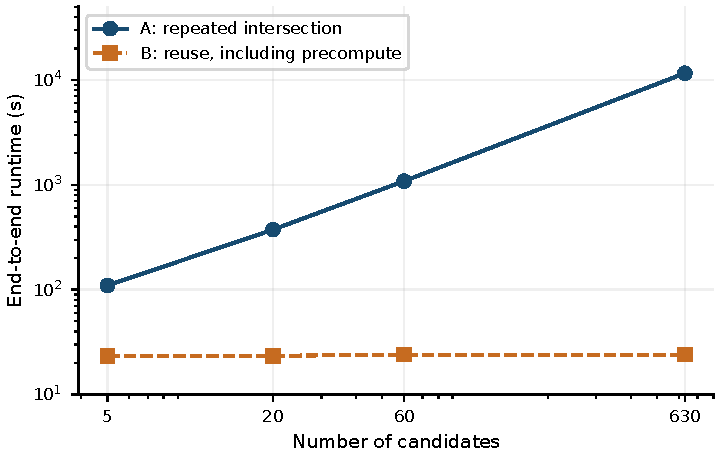
\includegraphics[width=\textwidth]{figures/runtime_publication.pdf}
\Description{Logarithmic plot of measured runtime against candidate count. A rises from approximately 110 seconds at five candidates to 11608 seconds at 630. B remains around 23 to 24 seconds, including precomputation.}
\caption{Measured same-primitive runtime comparison on the frozen canonical model. Both axes are logarithmic; points are medians of three repeats. Pointwise duration, metrics, score, rank and Pareto checks agree. The figure contains aggregate results only.}
\label{fig:runtime}
\end{figure}

This is an implementation comparison, not a general solver comparison. In particular, the repeated-intersection implementation is not a spatial-index baseline, and the experiment does not time equivalent Honeybee scenes against B. Cross-machine and cross-solver timings are excluded; superiority to other optimized implementations remains unmeasured.

Consistency with the frozen full-universe output is retained: $A/H/N$ differences are zero, maximum absolute $V$ and score differences are approximately $9.09\times10^{-13}$~m$^3$ and $4.44\times10^{-16}$, respectively, and the 630-candidate ranking is unchanged. These rounding-level checks concern the canonical model, not its fidelity to the physical site.

\subsection{Agreement within Preserved Cohorts}
Table~\ref{tab:agreement} separates the two cohorts and the three compared metrics. For low-sun-area reduction, the curated cohort has Spearman $\rho=0.999258$ and the coverage cohort $\rho=0.997668$. In the latter, 19 candidates agree exactly and one differs by 9~m$^2$, yielding MAE 0.45~m$^2$. This is an average candidate-aggregate error on a grid with 9~m$^2$ cell weights; it is not sub-grid spatial precision. Figure~\ref{fig:agreement} visualizes the same frozen aggregate comparison.

\begin{table}[tbp]
\caption{Descriptive same-metric agreement with archived Honeybee aggregates. Statistics are recomputed from frozen tables; no new cohort simulations are implied.}
\label{tab:agreement}\centering
\begin{tabular}{llrrr}\toprule
Cohort & Metric & Spearman $\rho$ & MAE & Exact matches\\\midrule
Curated ($n=23$) & $A$ (m$^2$) & 0.999258 & 0.391304 & 22/23\\
 & $H$ (h) & 0.991597 & 0.001177 & 3/23\\
 & $S$ & 0.999012 & 0.006933 & 3/23\\
Coverage ($n=20$) & $A$ (m$^2$) & 0.997668 & 0.450000 & 19/20\\
 & $H$ (h) & 0.999624 & 0.000295 & 9/20\\
 & $S$ & 1.000000 & 0.002139 & 9/20\\\bottomrule
\end{tabular}
\end{table}

\begin{figure}[tbp]\centering
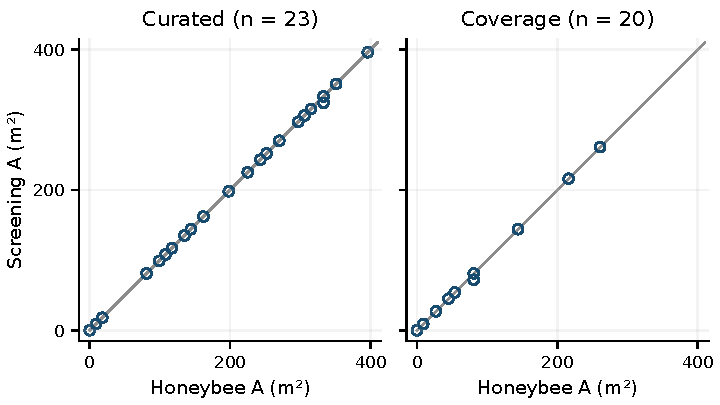
\includegraphics[width=\textwidth]{figures/agreement_publication.pdf}
\Description{Comparison of screening and archived Honeybee low-sun-area reductions, displayed separately for the curated 23 and coverage 20 candidate cohorts. Near-diagonal aggregate agreement does not establish site or pointwise equivalence.}
\caption{Low-sun-area agreement from frozen candidate aggregates. Each cohort remains separate. The coverage cohort's mean absolute difference of 0.45~m$^2$ arises from one 9~m$^2$ discrepancy among 20 candidates.}
\label{fig:agreement}
\end{figure}

Coverage-cohort score ranks agree perfectly, but the score values do not: MAE is 0.002139 and only 9 of 20 scores agree exactly. Shared $V$, constant $N$ and different effective solar vectors limit interpretation: perfect score-rank agreement does not validate four independent criteria or establish 100\% predictive accuracy.

Tie handling materially affects the top-five $A$ comparison within the 20-candidate coverage cohort. Here overlap is divided by five for exact-five sets. The retained legacy source-order result of 0.8 becomes 1.0 under the specified natural-pair exact-five rule, while including all boundary ties produces sets of six and seven candidates. This is a change in set definition, not an improvement in the physical model. We consequently avoid presenting a single top-five overlap as a universal selection guarantee. Likewise, an older correlation that compared score ranks to area ranks is not compared to the present same-metric correlations as evidence of progress.

\subsection{Translation Failure and Controlled Correction}
Four of five historical translations fail the solid-containment check. In C9/C24 and C13/C24, rays that were clear in the baseline intersect upper walls of C24 outside its original footprint. Each of these scenes has four worsened receiving points and 9~m$^2$ of newly low-sun grid area in the retained historical result. The actual ray hits identify added obstructions as the cause. Synthetic tests had also exposed hole-handling and silent-face risks, but the canonical site has no holes and the six archived face dictionaries regenerate exactly; those synthetic defects are not asserted as the cause of this case.

The four contained corrections have no adverse visibility events, worsened receiving points or newly low-sun grid area on the fixed model, rays and grid. Figure~\ref{fig:translation} retains the before/after distinction. Low-sun-area reduction changes from 342 to 351~m$^2$ for C9/C24 and from 207 to 216~m$^2$ for C13/C24. C9/C15 and C6/C33 remain at 342 and 18~m$^2$. The already-contained C9/C13 remains at 333~m$^2$ through reuse of its unchanged historical result, not an additional correction run.

\begin{figure}[tbp]\centering
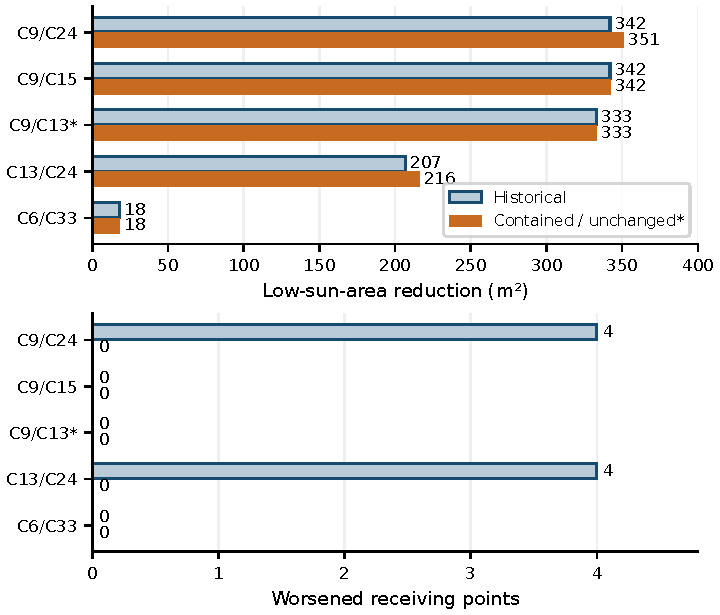
\includegraphics[width=\textwidth]{figures/translation_publication.pdf}
\Description{Five paired historical and corrected displays. C9/C24 and C13/C24 improve area reduction by nine square metres and reduce worsened points from four to zero. The C9/C13 corrected display reuses an unchanged historical result.}
\caption{Controlled translation recheck. Top: low-sun-area reduction relative to baseline. Bottom: worsened receiving-point count. Four corrections are newly simulated; C9/C13 is already contained and reuses its unchanged result. The historical adverse results remain visible; the comparisons are not volume matched.}
\label{fig:translation}
\end{figure}

For any translated solid, the signed net union-volume reduction is $|\Omega_0|-|\Omega_c|$. For a noncontained legacy solid, this equals removed baseline volume minus added outside volume; it is not gross removed material. Table~\ref{tab:volumes} shows why containment correction must not be called a volume-matched comparison. Nominal rule budgets, rule-solid net union-volume reduction and translated-solid net union-volume reduction differ. C6/C33 is particularly informative: its nominal additive proxy is 5,583.055~m$^3$, while uniform-rule net union-volume reduction is 1,909.864~m$^3$ and corrected translation net union-volume reduction is 2,554.767~m$^3$. These quantities characterize the frozen approximate solids, not verified demolition or construction quantities. Similar area outcomes do not imply geometrically equivalent interventions.

\begin{table}[tbp]
\caption{Volume distinctions in the canonical model (m$^3$). The nominal column is additive per building; other columns use signed whole-scene net union-volume reductions. C9/C13's correction column reuses its already-contained result.}
\label{tab:volumes}\centering
\begin{tabular}{lrrrr}\toprule
Pair & Nominal rule & Rule union & Legacy union & Corrected union\\\midrule
C9/C24 & 5,551.333 & 5,470.406 & 5,259.615 & 5,474.582\\
C9/C15 & 3,127.755 & 3,065.681 & 2,927.693 & 2,937.931\\
C9/C13 & 2,975.156 & 2,918.246 & 2,785.422 & 2,785.422\\
C13/C24 & 3,863.880 & 3,726.044 & 3,534.257 & 3,749.224\\
C6/C33 & 5,583.055 & 1,909.864 & 2,553.509 & 2,554.767\\\bottomrule
\end{tabular}
\end{table}

\FloatBarrier
\section{Discussion and Limitations}
\subsection{Implications for Decision Support}
The workflow separates three decisions that should not be collapsed into a single score.\aidraft{} First, exhaustive screening identifies preferred candidates within the declared rule universe. Reuse makes that comparison less expensive without introducing a new approximation relative to the common primitive. Second, the preference score and two-objective Pareto view organize alternatives under explicit criteria; they do not determine which criteria stakeholders should value. Third, the translation check tests whether the constructed geometry preserves the intended subtraction before its performance is interpreted.

This separation changes how a favorable result should be used. A highly ranked rule candidate warrants further examination, not automatic acceptance of a generated solid. The historical added-wall failure demonstrates why downstream feasibility must be checked independently of ranking. Containment is a necessary consistency check for a pure-subtraction interpretation; it is not a complete feasibility certificate. Actual removal cost, structural safety, legal rights and regulatory acceptability still require appropriate quantities, verified boundaries and professional review.

The practical value is therefore a reproducible shortlist with explicit reasons to accept, reject or revisit a translation. Retaining failed and corrected outcomes makes the decision traceable and prevents a geometric repair from being misrepresented as an improvement in the original ranking model. Extensions to another geometry, height rule or solar protocol require new blocker contributions and renewed checks; the present implementation comparison cannot establish their performance in advance.

\subsection{Threats to Validity}
\paragraph{Canonical geometry.} DXF component-bounding-box unions, shared components, overlapping footprints and OBJ disagreements limit external validity. Reproducing this model across implementations does not establish as-built fidelity. Revised boundaries would define a new input version requiring renewed evaluation; current cohort agreement cannot be transferred without evidence.

\paragraph{Restricted physical scope.} A single day, 16 samples, a 3~m grid, a 0.1~m receiving height and assumed north delimit the results. Threshold counts may change discontinuously near 3~h. Constant WEA inputs are not measured meteorology; indoor daylight, glare, annual energy and regulatory compliance are outside scope. Different pvlib and Ladybug rays preclude an identical-astronomical-input interpretation of cross-route agreement.

\paragraph{Comparison design.} The timing experiment controls the primitive and single-thread execution but covers one model and two implementations without spatial indexing. Three repeats do not characterize hardware populations or arbitrary polygons. Analytic blocker storage is not measured peak memory. Indexed and compiled baselines with identical accounting remain necessary for broader efficiency claims.

\paragraph{Cohorts and metrics.} Curated review and outcome-blind coverage serve different purposes and remain separate. Neither is a random multi-site sample. Shared volume inputs, constant $N$, discretized area, ties and preference weights constrain the interpretation of rank agreement. Candidate-level aggregate errors can mask spatial differences. The frozen 20 were not selectively rerun after the translation audit because no shared receiver, temporal-parser or missing-face defect was found in the actual scenes. A newly demonstrated shared defect would require an affected-scope review rather than selective retention of favorable outputs.

\paragraph{Correction scope.} The four corrections support containment on the tested model and rays, not arbitrary imported meshes. Containment neither matches volumes nor establishes structural feasibility or preference. Decisions about physical removal costs require an audited quantity beyond the nominal $V$ proxy.

\subsection{Reproducibility and Responsible Release}
The evidence separates measured runtime, newly executed scene replays, frozen-table statistical recomputation and historical reused results. Run identifiers, source, configuration and input hashes, raw timing repeats, aggregate tables, equivalence checks, correction ledgers and figure-source manifests are retained. The recorded 112 passing integrated tests provide software regression evidence, not physical ground truth; failures and amendments are retained alongside them.

Raw CAD, DXF, SKP and OBJ inputs, receiver coordinates, WEA carriers, Honeybee models and Radiance intermediate data remain restricted. Figures in this manuscript show aggregate evidence without site geometry or receiver coordinates. No public artifact release or unrestricted replication right is asserted. Any external evidence package must be reviewed for rights and anonymity before distribution. This restriction limits independent reproduction of the site-specific experiment and should remain visible alongside the available aggregate and algorithmic detail.

\section{Conclusion}
A bounded solar-access screening problem can reuse exact building-level occlusion contributions while keeping its preference model and geometric limitations explicit.\aidraft{} On the frozen 45-building canonical model, all 630 pair candidates are evaluated with equivalent outputs by two same-primitive implementations. Three matched repeats yield median end-to-end times of 11,608.183~s for repeated intersection and 24.037~s for blocker reuse, including preparation. The resulting ratio is specific to those implementations and inputs.

Preserved cohorts show strong same-site aggregate agreement, while controlled replays locate outside-footprint obstructions and remove the observed adverse events in four contained corrections. The results support auditable screening, not as-built accuracy, volume-matched interventions or automatic design approval. Verified boundaries, broader site coverage and additional optimized baselines are the next substantive extensions.

\section*{AI-Assistance Disclosure}
An OpenAI assistant~\cite{openai2026} assisted with evidence organization, drafting and editing the abstract and Sections~1--8, mathematical presentation, table transcription, figure captions and alternative text, bibliography checking, and LaTeX build and quality-control scripts. The manuscript uses reported experimental measurements and frozen aggregates; no numerical observations were generated to fill missing evidence. The assistant also prepared publication-size plots from unchanged aggregate tables and assisted with a bounded literature-positioning and prose revision. The plots were regenerated from their recorded CSV inputs during revision; no physical simulation was rerun for that revision. These figures reproduce recorded evidence rather than generative illustrations. This statement describes the assistance used for the present draft. The exact underlying model/version was not recorded, so no model-version claim is made.

\FloatBarrier
\bibliographystyle{splncs04}
\bibliography{references}
\end{document}
